\subsection{Glyph: \glyph{Biological activity}}
\label{sec:af:biologicalActivity}

\SBGNAFLone uses one glyph to represent activities from all biological entities, collectively they are called \emph{biological activity}. The nature of the molecule that the activity comes from, eg., simple chemical or macromolecule, can be encoded in the \emph{units of information} (\sect{af:unitInfo}).

It should be noted that the \emph{biological activity} is not equivalent to a biological entity per se.  A biological activity can come from one biological entity, a part of an entity, or a combination of  them.  It is up to the users to determine how to represent it in their diagram.  For example, a protein kinase receptor such as an EGF receptor, has two activities, the binding activity that allows the extracellular part of the receptor to bind to the ligand, and the kinase activity that is capable of phosphorylating the downstream protein and initiating the intracellular signaling.  The user can choose to use two nodes to represent each activity, or to use one node to represent the overall "EGF receptor activity".

\begin{glyphDescription}

\glyphSboTerm SBO:0000412 ! biological activity

\glyphContainer An \glyph{biological activity} is represented by a rectangle, as shown in \fig{af:biologicalActivity}.

\glyphLabel An \glyph{biological activity} is identified by a label placed in an unbordered box containing a string of characters.  The characters can be distributed on several lines to improve readability, although this is not mandatory.  The label box must be attached to the center of the container.  The label may spill outside of the container.

\glyphAux A \glyph{biological activity} can carry a \glyph{unit of information} (\sect{af:unitInfo}), which can provide information such as the nature of the entity from which the activity originated.  Specific glyphs are used to represent different types of entities (\sect{af:unitInfo}).  The center of the bounding box of a \glyph{unit of information} is located on the mid-line of the border of the macromolecule.  The label in the \glyph{unit of information}, which is optional, indicates the name of the molecule where the activity comes from, as shown in \fig{af:EGFR}

\end{glyphDescription}

\begin{figure}[H]
  \centering
  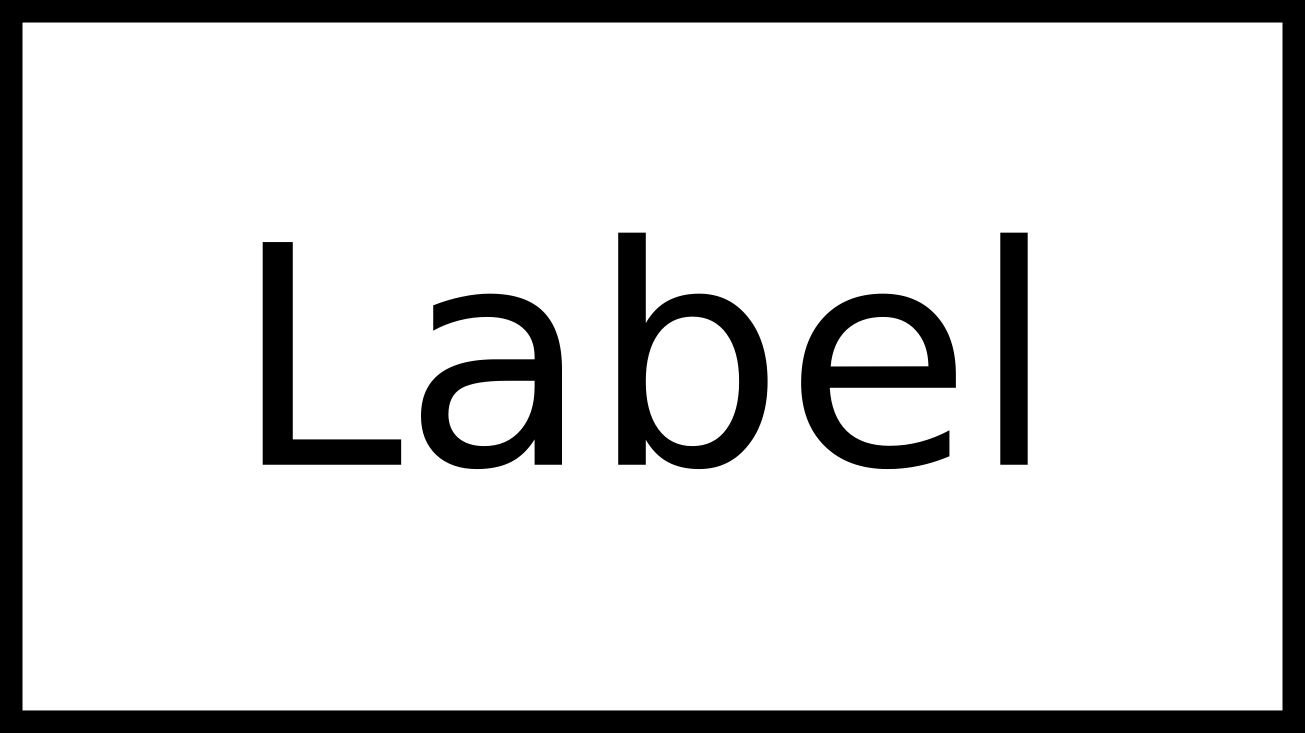
\includegraphics[scale=0.5]{images/biologicalActivity}
  \caption{The \AF glyph for \glyph{biological activity}.}
  \label{fig:af:biologicalActivity}
\end{figure}

\begin{figure}[H]
  \centering
  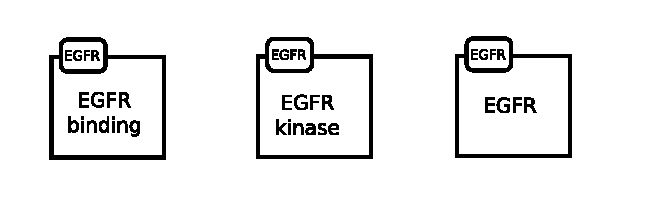
\includegraphics[scale = 1]{examples/EGFR}
  \caption{An example of \AF glyphs of EGFR activities.  Since EGFR protein has both binding and kinase activities, each of those activity can be represented by different nodes, labeled as \emph{EGFR binding} and \emph{EGFR kinase}.  One node can be used to represent the overall activity of \emph{EGFR}.  The label in the \glyph{unit of information} indicates the protein that the activities come from.  In this example, all three activities come from the same EGFR protein}
  \label{fig:af:EGFR}
\end{figure} 